\section{Virtuelles Filesystem}
\label{kap:vfs}
Dieses Kapitel beschreibt die Umsetzung des virtuellen Filesystems (VFS). Ziel der Umsetzung ist es, die in Kapitel~\ref{sec:problemstellung} beschriebenen Herausforderungen zu lösen. Im Folgenden werden zunächst die konzeptionellen Überlegungen vorgestellt, bevor auf die technische Umsetzung eingegangen wird.

\subsection{Lösungsansätze}
\label{sec:vfs-konzeption}
In diesem Abschnitt werden verschiedene Lösungsansätze zur Umsetzung des VFS vorgestellt und bewertet. Die Komponenten „Explorer“ und „Editor“ werden getrennt betrachtet, da ihre Aufgaben unterschiedlich sind. Zum Schluss folgt eine gemeinsame Betrachtung beider Komponenten.

\subsubsection{Explorer}
Wie bereits in Kapitel~\ref{kap:Architek} beschrieben, dient der Explorer der Navigation durch die Instanzen. Grundlage hierfür bildet das Datenbankschema. Vor der Umsetzung sind folgende konzeptionelle Fragen zu klären:
\begin{itemize}
  \item Wie wird die URI-Struktur generiert?
    \item Wie ist die Benutzeroberfläche gestaltet?
    \item Wie werden die Daten bereitgestellt?
    \item Wie werden Referenzen, Zyklen und Blattknoten beim Traversieren behandelt?
    \item Welche Funktionen bietet der Explorer und welche Einschränkungen bestehen?
\end{itemize}

\subsubsection*{URI Konzept}
\label{sec:urikonzept}
Eine Uniform Resource Identifier ist eine Zeichenfolge zur eindeutigen Identifikation und zur Beschreibung der hierarchischen Position einer Ressource. Aus einer URI lassen sich die Position einer Ressource innerhalb der Struktur sowie deren Beziehungen zu anderen Ressourcen ableiten~\cite{rfc3986}.

In dieser Arbeit werden URIs verwendet, um Instanzen eindeutig zu identifizieren, deren Beziehungen zueinander zu erkennen und sie in einer Baumstruktur im Filesystem abzubilden. Die Struktur einer URI ergibt sich, wie bereits in Abschnitt~\ref{sec:dynamischerAb} beschrieben, aus der Kombination des Namens eines Referenzfeldes und eines eindeutigen Bezeichners der Instanz. Damit jede Instanz innerhalb dieser Struktur eindeutig und zugleich verständlich benannt werden kann, wird das bisher vorgestellte Domänenmodell (siehe Kapitel~\ref{kap:dbschema}) um ein neues Feld erweitert: den „Slug“. Ein Slug ist eine eindeutige Bezeichnung vom Typ \texttt{string}, die für jede Instanz im Datenbankschema definiert werden muss. Der Slug wird beim Erstellen einer neuen Instanz im Explorer vergeben und entspricht dabei dem Namen des Ordners.

Die URI folgt einem festen Muster: Ungerade Segmente enthalten den Namen des Referenzfeldes aus dem Datenmodell, wobei der erste Buchstabe grossgeschrieben wird (z.B. wird aus „addressen“ immer „Addressen“). Gerade Segmente enthalten den Slug der zugehörigen Instanz. Einstiegspunkte (Roots) besitzen kein Referenzfeld, weshalb hier das im Schema definierte Label als erstes URI-Segment verwendet wird. Jeder Slug muss innerhalb seines Pfades eindeutig sein. Diese Eindeutigkeit stellt der Explorer beim Erstellen neuer Instanzen sicher und wird zusätzlich durch den VFS-Controller geprüft.

Ein Beispiel verdeutlicht diesen Aufbau: Erstellt ein Systemintegrator einen neuen Kunden mit dem Ordnernamen „max“, so ergibt sich die URI \texttt{/Customers/max}. Dabei ist „Customers“ das Label des Root-Typs, und „max“ der eindeutig vergebene Slug der Instanz.


%Gehört in Umsetzung
%Wie in Abschnitt~\ref{sec:Datenzugriff} beschrieben, wird die URI beim Erstellen einer Instanz als Alias in der Selva-Datenbank gespeichert. Dafür wird die entsprechende Alias-Funktion der Datenbank genutzt. Dadurch ist jede Instanz direkt über ihre URI abrufbar. Aus dem URI-Verlauf lassen sich zudem abhängige Kindinstanzen ableiten. Die URI-Struktur reduziert somit die Komplexität bei der Datenbereitstellung im virtuellen Filesystem und vereinfacht die Implementierung des Language Servers.


%Jede URI ist eindeutig und wird als Referenzpfad verwendet. In der Datenbank dient sie gleichzeitig als Alias, um eine  Identifikation und Navigation zu ermöglichen (siehe Abschnitt~\ref{sec:Datenzugriff}).

%Zudem bildet das URI-Konzept die Grundlage für die Implementierung des Language Servers (siehe Kapitel~\ref{sec:lsp}). Der Language Server kennt ausschliesslich die URI sowie den Inhalt der aktuell im Editor geöffneten Datei. Da jede Instanz eindeutig über ihre URI identifiziert wird, reduziert sich die Komplexität bei der Implementierung des Language Servers deutlich. Zusätzliche interne Identifikatoren müssen im Editor nicht verwaltet werden.

\subsubsection*{Benutzeroberfläche}
\label{par:uiExploerer}
Die Benutzeroberfläche basiert auf der integrierten Explorer-Ansicht von Visual Studio Code. Der Explorer stellt grundlegende Dateioperationen wie das Erstellen, Umbenennen, Löschen und Verschieben von Dateien und Ordnern zur Verfügung und ermöglicht die Navigation innerhalb der Verzeichnisstruktur. Da diese Aktionen systemseitig nicht deaktiviert werden können, ergeben sich Einschränkungen bei bestimmten Nutzeraktionen. Diese werden im Abschnitt~\ref{sec:Nutzeraktionen} näher erläutert. Eine zusätzliche technische Begrenzung besteht darin, dass die Editor-Komponente nicht um weitere Bedienelemente, wie beispielsweise Schaltflächen, erweitert werden kann. Individuelle Icons innerhalb der Explorer-Ansicht wären technisch umsetzbar, wurden jedoch im Rahmen dieser Arbeit nicht implementiert.

Zur Verdeutlichung wird die Darstellung des Explorers anhand des zuvor eingeführten Domänenmodells (siehe Abschnitt~\ref{kap:dbschema}) in Abbildung~\ref{fig:explorer-ui} gezeigt.

\begin{figure}[H]
  \centering
  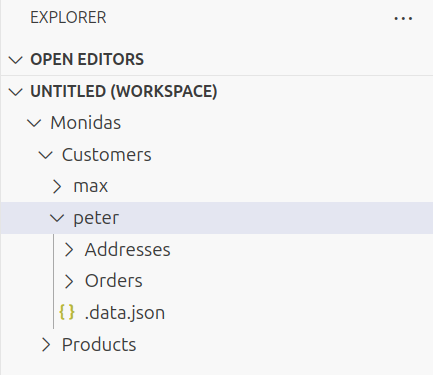
\includegraphics[width=0.4\linewidth]{explorer-ui.png}
  \caption{}
  \label{fig:explorer-ui}
\end{figure}

Wie aus der Abbildung ersichtlich, entspricht die Struktur des Explorers dem zuvor eingeführten URI-Konzept (siehe Abschnitt~\ref{sec:vfs-konzeption}). Auf oberster Ebene befinden sich die bekannten Root-Ordner. Darunter folgen Ordner für einzelne Instanzen. Beim Öffnen einer Instanz wird eine Datei mit dem Namen \texttt{.data.json} angezeigt, welche die Instanzdaten im JSON-Format enthält. Zusätzlich erscheinen Ordner, deren Bezeichnungen sich unmittelbar aus den Referenzfeldern des Datenbankschemas ableiten. Die genaue Bedeutung und Nutzung der Datei wird in Abschnitt~\ref{sec:Editor} erläutert.

Beim Aufklappen der Ordner ergeben sich spezielle Darstellungs- und Navigationsfälle, welche gesondert evaluiert wurden. Diese werden in Abschnitt~\ref{sec:referenz-zyklusbehandlung} und Abschnitt~\ref{sec:blattknoten} erläutert.

Für eine einheitliche Darstellung im weiteren Verlauf der Arbeit werden die Begriffe «Root-Ordner» für oberste Einstiegspunkte, «Referenzordner» für aus Referenzfeldern abgeleitete Ordner und «Instanzordner» für Ordner der Instanzen verwendet.

\newpage
\subsubsection*{Bereitstellung der Daten}
Die Bereitstellung der Daten beschreibt, wie die im Explorer benötigten Daten technisch geladen und dargestellt werden. Nutzeraktionen, beispielsweise das Öffnen oder Aufklappen eines Ordners im Explorer, lösen Datenanfragen durch die VFS-Extension aus. Für diese Datenbereitstellung wurden zwei Lösungsansätze untersucht: das Pull-Prinzip und das Push-Prinzip.

Beim Pull-Prinzip fordert die VFS-Extension die Daten erst dann vom VFS-Controller an, wenn eine entsprechende Nutzeraktion erfolgt. Ein wesentlicher Vorteil hierbei ist, dass tatsächlich benötigte Daten geladen werden und der Datenaustausch klar steuerbar bleibt. Ein Nachteil liegt allerdings darin, dass externe Datenänderungen, wie etwa Änderungen durch andere Nutzer oder Prozesse im Hintergrund, nicht erkannt werden, da Daten nur auf Anfrage hin aktualisiert werden.

Alternativ wurde das Push-Prinzip untersucht. Bei diesem Ansatz werden Datenänderungen vom Controller proaktiv an die VFS-Extension gesendet. Dabei abonniert die VFS-Extension Benachrichtigungskanäle, die sie über Datenänderungen informieren. Jedoch zeigten sich bei diesem Ansatz Schwierigkeiten, da interne Aktionen wie das erneute Rendern sämtlicher geöffneter Ordner im Explorer komplexe Logiken zur Verwaltung der Subscriptions erfordern. Dies führte zu erhöhtem Aufwand und Implementierungsschwierigkeiten.

Aufgrund der geringeren Komplexität, besseren Steuerbarkeit und bewussten Nichtberücksichtigung von Multi-User-Szenarien wurde das Pull-Prinzip gewählt. Zukünftige Erweiterungen könnten dieses Prinzip bei Bedarf ergänzen, indem wichtige externe Änderungen über gezielte, eventbasierte Push-Benachrichtigungen übertragen werden. Technische Einzelheiten zur Umsetzung sind im Abschnitt \ref{subsec:explorer-baum} beschrieben.


\subsubsection*{Referenz- und Zyklusbehandlung}
\label{sec:referenz-zyklusbehandlung}
Beim Navigieren im Explorer können Instanzen andere Instanzen referenzieren. Dadurch stellt sich die konzeptionelle Frage, wie der Explorer beim Aufklappen von Ordnern mit solchen Referenzen umgehen soll. Ein Sonderfall entsteht, wenn dieselbe Instanz innerhalb eines Pfades erneut vorkommt. Man spricht dann von einem \textit{Zyklus}. 

Für die Behandlung dieser Situationen wurden zwei Lösungsansätze geprüft:

Beim ersten Ansatz werden zyklische Referenzen vollständig aufgeklappt dargestellt, wodurch dieselbe Instanz mehrfach im Explorer erscheint. Der Vorteil dieses Ansatzes besteht in einer flexiblen und uneingeschränkten Navigation für den Benutzer. Während der Evaluierung zeigte sich allerdings, dass die technische Komplexität der VFS-Extension dadurch erheblich zunimmt. Zwar ermöglichen interne IDs eine eindeutige Identifikation der Instanzen, zusätzlich wäre jedoch ein Mechanismus für symbolische Verknüpfungen („Softlinks“) erforderlich. Dieser würde sicherstellen, dass Änderungen an einer Instanz konsistent auf alle mehrfach dargestellten Kopien übertragen werden.

Der zweite Lösungsansatz verhindert von vornherein das Aufklappen referenzierter Instanzen im Explorer. Sobald eine bestehende Instanz erneut referenziert wird, lässt die Anwendung kein weiteres Aufklappen zu, wodurch Zyklen grundsätzlich vermieden werden. Ein wesentlicher Vorteil ist die deutlich geringere technische Komplexität, da Mehrfachdarstellungen und deren Synchronisation vollständig entfallen. Die dadurch entstehende Einschränkung in der Navigation wird durch eine ergänzende „Jump-to-Definition“-Funktion kompensiert, die Nutzern das direkte Navigieren zur ursprünglichen Instanz ermöglicht. Die Umsetzung dieser Funktion wird im Abschnitt zum Language Server ausführlich erläutert.

\subsubsection*{Blattknoten}
\label{sec:blattknoten}
Im Rahmen der konzeptionellen Darstellung im Explorer stellt sich die Frage, wie Instanzen dargestellt werden sollen, die laut Datenbankschema nur einmal pro übergeordnetem Objekt erstellt werden können. Im aktuellen Domänenmodell wurde beispielsweise festgelegt, dass ein Kunde mehrere Adressen erstellen darf. Falls jedoch das Schema so definiert wäre, dass ein Kunde nur exakt eine Adresse erstellen kann, ergibt sich die Frage, wie diese einzelne Instanz im Explorer dargestellt werden soll. \footnote{Die Abbildungen~\ref{fig:noinline} und~\ref{fig:inline} sind hypothetischen und entsprechen nicht dem Domänenmodell aus Abschnitt \ref{abb:domaenenmodell}.}


Dafür wurden zwei mögliche Lösungsansätze betrachtet:

\textbf{Reguläre Darstellung}\\
Blattknoten werden analog zu regulären Instanzen als separate, aufklappbare Ordner dargestellt. Dies hätte den Vorteil, dass keine zusätzliche technische Logik notwendig wäre, um Blattknoten speziell zu erkennen. Als Nachteil entsteht jedoch eine erhöhte Navigationskomplexität, da zusätzliche Hierarchieebenen entstehen.

\textbf{Inline-Darstellung}\\
Blattknoten werden direkt innerhalb der Parent-Instanz dargestellt, wodurch eine zusätzliche Navigationsebene entfällt. Diese Variante verbessert die Übersichtlichkeit deutlich. Nachteilig ist allerdings der erhöhte Implementierungsaufwand, da Blattknoten explizit erkannt und gesondert behandelt werden müssen. Zudem ist für Nutzer erst nach dem Öffnen der Parent-Instanz ersichtlich, ob ein Blattknoten überhaupt existiert.

\begin{figure}[H]
    \centering
      \begin{minipage}{0.45\textwidth}
        \centering
        \includegraphics[width=1\linewidth]{noinline.png}
        \caption{Reguläre Darstellung}
        \label{fig:noinline}
    \end{minipage}\hfill
    \begin{minipage}{0.45\textwidth}
        \centering
        \includegraphics[width=1\linewidth]{inline.png}
        \caption{Inline-Darstellung}
        \label{fig:inline}
    \end{minipage}
\end{figure}

Aufgrund der verbesserten Übersichtlichkeit und der Reduktion unnötiger Navigationsschritte wurde trotz des höheren Implementierungsaufwands die Inline-Darstellung innerhalb der Datei gewählt. Für eine mögliche Erweiterung der Anwendung wäre es denkbar, dem Nutzer die Wahl der bevorzugten Darstellung zu überlassen, beispielsweise über eine entsprechende Einstellung in der Benutzeroberfläche.

\newpage
\subsubsection*{Nutzeraktionen im Explorer}
\label{sec:Nutzeraktionen}
Wie in Abschnitt~\ref{par:uiExploerer} beschrieben, stehen im Explorer die Standardaktionen eines Filesystems zur Verfügung. Da die Struktur des Explorers direkt durch das zugrunde liegende Datenbankschema bestimmt wird, sind einzelne Aktionen gezielt eingeschränkt. Im Folgenden wird erläutert, wie diese Aktionen durchgeführt werden, auf welche Ordner und Dateien sie angewendet werden können und weshalb dabei bestimmte Einschränkungen erforderlich sind.

\textbf{Ordner erstellen}\\
Mit dem Erstellen eines neuen Ordners leitet man im Monidas CAN den Erstellprozess einer neuen Instanz ein. Wie ein Erstellprozess definiert ist, wird im Abschnitt~\ref{sec:Editor} beschrieben, da dieser Abhängigkeiten zum Editor aufweist. Aus diesem Grund ist das Erstellen nur auf Ebene der Root- und Referenzordner möglich. Auf Instanzordner-Ebene ist das Erstellen dagegen nicht erlaubt, da jede Instanz zwingend auf einer definierten Entität im Datenbankschema basieren muss. Versuche, auf Instanzordner-Ebene einen Ordner zu erstellen, werden mit einer Popup-Fehlermeldung abgelehnt.

\textbf{Datei erstellen}\\
Das Erstellen einer Datei ist auf keiner Ordnerebene erlaubt. Die einzige erlaubte Datei ist die von der VFS-Extension bereitgestellte data.json. Diese Datei stellt die Daten einer Instanz zur Bearbeitung im Editor bereit. Da das virtuelle Filesystem keine lokalen Dateien speichert, werden Instanzdaten erst beim Zugriff aus der Datenbank geladen. Zusätzliche Dateien hätten keinen Bezug zum definierten Datenbankschema und könnten somit nicht von der Anwendung verarbeitet oder verwaltet werden. Solche Dateien wären wirkungslos für die Datenverwaltung und daher unnötig. Aus diesem Grund werden Versuche, weitere Dateien zu erstellen, abgelehnt. Dem Benutzer wird eine Popup-Fehlermeldung angezeigt.

\textbf{Umbenennen}\\
Nur Instanzordner dürfen umbenannt werden. Root- und Referenzordner haben feste Namen aus dem Datenbankschema und dürfen daher nicht geändert werden. Auch die Datei data.json darf nicht umbenannt werden, da sie als eindeutiger Zugriffspunkt auf die Instanzdaten dient. Ein Umbenennen würde den Datenzugriff verhindern. Unzulässige Umbenennungen werden mit einer Popup-Fehlermeldung abgelehnt.

%Beim Umbenennen eines Instanzordners verändert sich der Slug und somit auch die eindeutige URI der Instanz. Dabei wird das Feld aliases, welches die URI speichert, angepasst und alle abhängigen URIs aktualisiert. „Abhängige URIs“ sind URIs von Instanzen, die auf die umbenannte Instanz verweisen.

\textbf{Löschen}\\
Ein Löschvorgang ist, analog zur Umbenennung, nur auf Instanzordnern zulässig. Root- und Referenzordner sowie die Datei \texttt{data.json} sind dagegen fest vorgegeben und dürfen nicht gelöscht werden. Aufgrund der Integration in das VS-Code-Filesystem erscheint bei jedem Löschversuch ein Bestätigungsdialog, welcher sich nicht deaktivieren lässt. Daraus entsteht der Nachteil, dass selbst bei unzulässigen Löschaktionen zuerst der Bestätigungsdialog bestätigt werden muss. Erst danach folgt die eigentliche Fehlermeldung, die ebenfalls als Dialog und nicht als einfache Popup-Meldung dargestellt werden kann.

Anzumerken ist auch, dass in dieser Arbeit keine Löschregeln (Delete-Policies) berücksichtigt wurden. Solche Regeln bestimmen, ob ein Objekt gelöscht werden darf, wenn andere Objekte darauf verweisen. Selva unterstützt diese Funktionalität nicht. Colomba Link bietet zwar eine eigene Datenbank-Implementierung, doch diese ist derzeit nicht URI-kompatibel. Da Colomba Link plant, diese Erweiterung selbst vorzunehmen, wurde bewusst auf eine eigene Umsetzung verzichtet.

\subsubsection*{Verschieben}
Das Verschieben von Ordnern und Dateien wird auf keiner Ordnerebene unterstützt. Theoretisch möglich wäre das Verschieben eines Instanzordners zwischen Referenzordnern desselben Entitätstyps. Ein Beispiel hierfür wäre das Verschieben der Heimadresse des Kunden \texttt{max} in den Adressordner des Kunden \texttt{peter}:

\begin{verbatim}
/Customers/max/Addresses/homeAddress → /Customers/peter/Addresses/
\end{verbatim}

Eine Voraussetzung hierfür wäre, dass keine anderen Instanzen auf die verschobene Instanz verweisen. Die Implementierung einer solchen Prüfung ist komplex und konnte im Rahmen dieser Arbeit zeitlich nicht berücksichtigt werden. Aus diesem Grund wird das Verschieben generell verhindert und jeder Versuch mit einer Fehlermeldung abgelehnt. Dasselbe gilt analog auch für die Aktion „Kopieren“.


\subsubsection{Editor}
\label{sec:Editor}
Während der Explorer die Navigation durch Instanzen ermöglicht, dient der Editor der Erstellung und Bearbeitung dieser Instanzen. Vor der Umsetzung sind folgende konzeptionelle Fragen zu klären:

\begin{itemize}
\item Warum erfolgt die Bearbeitung der Instanzdaten über eine (\texttt{.data.json}) Datei?
\item Wie werden Instanzen im Editor dargestellt?
\item Wie beeinflusst die Inline-Darstellung im Explorer das Bearbeitungskonzept im Editor?
\item Welche Validierungen sind erforderlich?
\item Welche Aufgaben übernimmt der Editor nicht?
\end{itemize}

\subsubsection*{Dateiformat}
Die Entscheidung, Instanzdaten pro Instanz in genau einer Datei im JSON-Format (.data.json) bereitzustellen, basiert auf konzeptionellen und technischen Gründen. Die Verwendung genau einer Datei pro Instanz reduziert die Komplexität bei der Navigation sowie der Bearbeitung der Instanzen, da sämtliche Daten an einer Stelle zusammengefasst sind. Dies verhindert, dass Nutzende während der Bearbeitung zwischen mehreren Dateien wechseln müssen.

Das JSON-Format wurde gewählt, weil es strukturierte Daten übersichtlich darstellt und von Menschen sowie Maschinen einfach verarbeitet werden kann. Aufgrund seiner weiten Verbreitung und Standardisierung eignet es sich besonders für den Datenaustausch zwischen den Komponenten der Anwendung.

Ein weiterer Grund für die Wahl des JSON-Formats ist dessen bisherige Verwendung innerhalb der Monidas-Plattform. Bereits bestehende Komponenten der Plattform nutzen JSON zur Verwaltung und Konfiguration von Sensor- und Monitorparametern (siehe Abschnitt \ref{kap:konf}). Diese Konsistenz vereinfacht die Integration und Wartbarkeit der Lösung.

Technisch ermöglicht JSON eine direkte Bearbeitung im Editor von Visual Studio Code ohne zusätzlichen Implementierungsaufwand. Zudem stellt JSON die Grundlage für Editorfunktionen wie Validierung und Autovervollständigung dar, die über den Language Server umgesetzt werden (siehe Kapitel \ref{kap:lsp}).

\newpage
\subsubsection*{Benutzeroberfläche}
Die Benutzeroberfläche zur Bearbeitung der Instanzdaten basiert auf der integrierten Editor-Komponente von Visual Studio Code. Beim Öffnen der Datei .data.json werden sämtliche Felder einer Instanz angezeigt. Diese Felder entsprechen direkt den im Datenbankschema definierten Feldern und werden im Editor stets nach einer festgelegten Reihenfolge dargestellt, um eine konsistente Bearbeitung zu gewährleisten.

Das Feld slug, welches als Ordnername einer Instanz im Explorer verwendet wird, ist im Editor nicht sichtbar. Änderungen am slug erfolgen über die Umbenennungsfunktion des Explorers (siehe Abschnitt~\ref{sec:Nutzeraktionen}). Diese bewusste Trennung vermeidet zusätzlichen Aufwand, welcher durch notwendige Validierungen und Synchronisationsprozesse zwischen Explorer und Editor entstehen würde.

Die im Editor dargestellten Felder entsprechen den im Datenbankschema definierten Datentypen (siehe Abschnitt \ref{sec:Datenzugriff}). Einfache Datentypen (string, boolean, number) werden als entsprechende JSON-Werte dargestellt. Referenzfelder (reference, references) werden grundsätzlich mit einer Kombination aus eindeutiger ID und dem slug der referenzierten Instanz angezeigt. Diese Darstellung dient als Hinweis auf die Herkunft der referenzierten Instanz und unterstützt die spätere Editorfunktionalität des Language Servers, zur Navigation („Jump-to-Definition“). Weiterführende Informationen zur Darstellung und den unterstützenden Editorfunktionen werden im Kapitel zur Editorunterstützung mit LSP detailliert beschrieben (siehe Kapitel \ref{kap:lsp}).

Eine Ausnahme zur oben beschriebenen Darstellung bilden Blattknoten, deren Darstellung und Erstellung im Editor im folgenden Abschnitt näher erläutert werden (siehe Abschnitt \ref{sec:EDblattknoten}).

\begin{figure}[H]
\centering
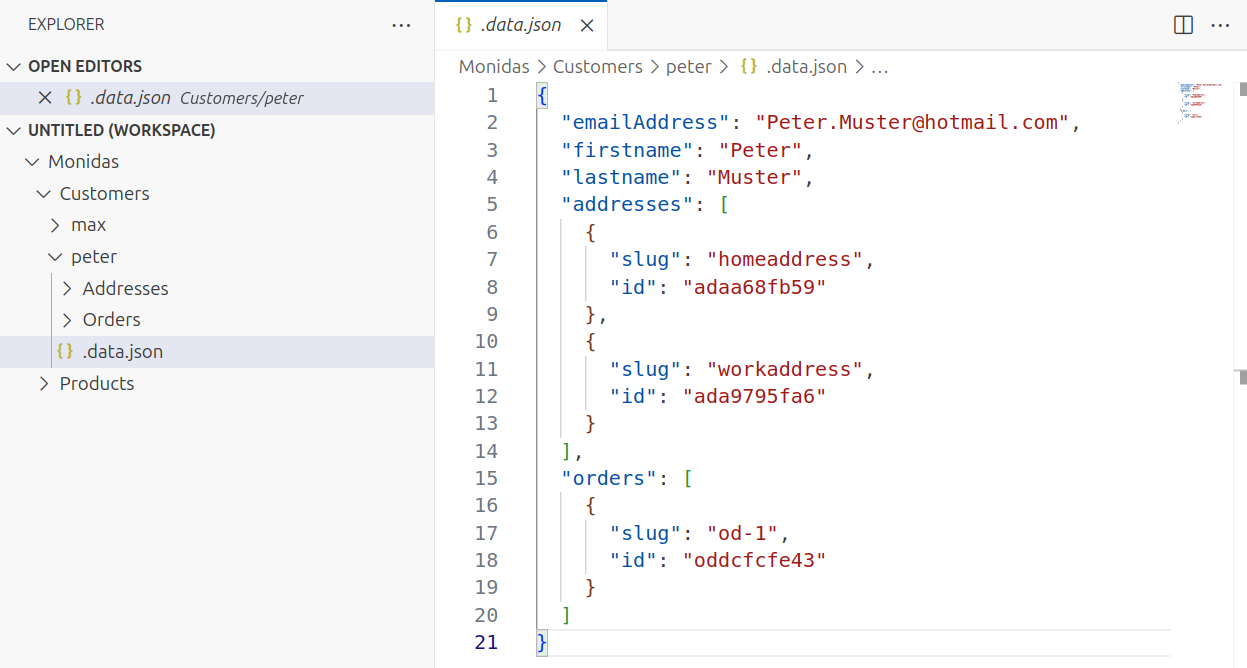
\includegraphics[width=0.9\linewidth]{editor-ui.png}
\caption{Darstellung der Instanzdaten im Editor}
\label{fig:editor-ui}
\end{figure}

\newpage
\subsubsection*{Blattknoten}
\label{sec:EDblattknoten}
Wie bereits in Abschnitt \ref{sec:blattknoten} beschrieben, weicht die Darstellung und Bearbeitung von Blattknoten im Editor von der Standarddarstellung ab. Im Folgenden werden diese Unterschiede detailliert erläutert.

\begin{figure}[H]
\centering
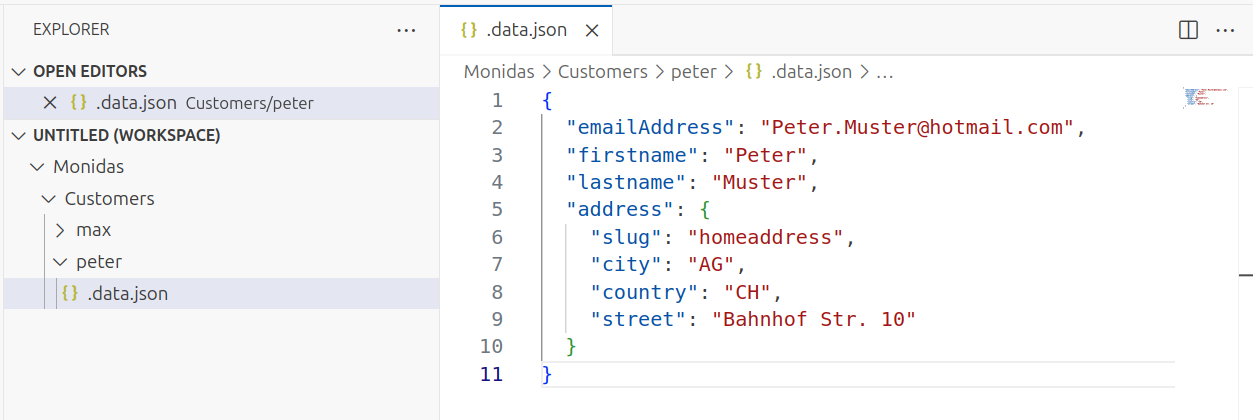
\includegraphics[width=1\linewidth]{inlineEditor.png}
\caption{}
\label{fig:inlineEditor}
\end{figure}

\subsubsection*{Validierung}

\subsubsection*{Abgrenzung}


\subsubsection{Zusammenspiel Explorer und Editor}


\subsection{Umsetzung}
\label{sec:vfs-umsetzung}


\subsubsection{Aufbau des Explorer-Baums}
\label{subsec:explorer-baum}


\subsubsection{Editor-Integration}
\label{subsec:editor-integration}

\subsubsection{Datenvalidierung}
\label{subsec:vfs-validierung}

\subsubsection{Benachrichtigungen und Nutzerfeedback}
\label{subsec:vfs-benachrichtigungen}

\subsection{Bewertung der Lösung}
\label{sec:vfs-bewertung}

%Alle im Explorer dargestellten Ordner sind virtuell und werden erst beim Aufklappen durch den Nutzer geladen („Pull-Prinzip“, siehe Abschnitt~\ref{sec:vfs-konzeption}). Bereits geladene Daten werden temporär im Cache gehalten und erst bei Änderungen, beispielsweise nach einer Umbenennung, erneut abgerufen. Die Datei \texttt{.data.json} enthält beim ersten Anzeigen noch keine Daten. Erst beim Öffnen der Datei im Editor werden die Instanzdaten abgerufen und angezeigt. Eine dauerhafte lokale Speicherung findet nicht statt.